\documentclass[11pt]{article}

\usepackage{tikz}
\usepackage{tikz-qtree}
\usepackage{algorithm}
\usepackage[noend]{algpseudocode}

% \pagestyle{empty}
% \textwidth 165mm
% \textheight 252mm
% \topmargin -13mm
% \oddsidemargin -2mm
% \evensidemargin -2mm
\renewcommand{\baselinestretch}{1.03}
\newcommand{\id}[1]{\mbox{\textit{#1}}}
\newcommand{\tuple}[1]{\langle #1 \rangle}

\begin{document}

\begin{center}
{\sc The University of Melbourne
\\
School of Computing and Information Systems
\\
COMP90038 Algorithms and Complexity}
\bigskip \\
{\Large\bf Assignment 2, Semester 2, 2017}
\bigskip \\
{Student Name: XX

Student No.: XXXXXX}
\end{center}
\section*{My Answers}
\subsection*{Challenge 1 \hfill {\small (1 mark)}}
\begin{center}
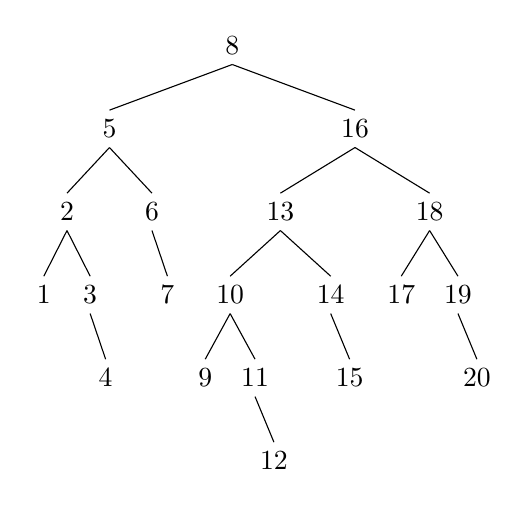
\begin{tikzpicture}
\tikzset{
    no/.style={draw=none}
}
\Tree [.8 [.5 [.2 1 [.3 \edge[no]; {} {4} ] ] [.6 \edge[no]; {} {7} ] ]
          [.16 [.13 [.10 [.9 ] [.11 \edge[no]; {} {12} ] ] [.14 \edge[no]; {} {15} ] ]
               [.18 [.17 ] [.19 \edge[no]; {} {20} ] ] ] ]
\end{tikzpicture}
\end{center}
% this is the original tree drawer of tikz, which cannot automatically adjust the position
% of node.
% \begin{tikzpicture}
%     [level 1/.style={sibling distance=6cm},
%     level 2/.style={sibling distance=2.5cm}, 
%     level 3/.style={sibling distance=2.5cm}, 
%     level distance=1cm,]
%     \node {8}
%         child {node {5}
%             child {node {2}
%                 child {node {1}}
%                 child {node {3}}}
%             child {node {6}
%                 child {node {}}
%                 child {node {7}}}}
%         child {node {16}
%             child {node {13}}
%             child {node {18}}
%         };
% \end{tikzpicture}

\subsection*{Challenge 2 \hfill {\small (2 mark)}}
Maybe the Right Answer: $d_{\mathit{worst}} = 5$, drops in sequence: $5, 9, 12, 14$.
\\
Wrong Answer:
According to the following strategy, in the worst case, $d = 6$.

Now Dr. Luator have 2 detectors to use in the test, she could start the test from not level 1
but level 4. After the dropping the first detector, if it's safe, she should shift 4 levels and 
drop on level 8, if safe once again, shift to and drop on level 12, and so forth.
When she reaches level 15 and there's no more room for a 4-level-shifting,
Dr. Luator should drop the first detector on level 15. If the first detector remains safe in all
these tests, then level 15 is the safe limit.

If the first detector breaks in any of the above tests, for example, on level 4,
then she should drop the second detector in the brute force way from level 1 to level 3.
Similarly, if the first detector, say, breaks on level 12, Dr. Luator should drop the second one
in brute force way, starting from level 9 until level 11. The reason she starts from level 9 is
that she already tested on level 8 and the first detector is safe, so all the levels before level 8
is ensured to be safe. If the second detector remains safe in the brute force way test,
then the safe limit should be the latest drop of the first detector.
If the second detector breaks, then the safe limit is the last drop of the second detector.

When using this startegy, in the worst case, the safe
limit floor $n$ should be $10, 11, 13, or 14$, and the drop $d$ should be $6$.

%\pagebreak
\subsection*{Challenge 3 \hfill {\small (3 mark)}}
\begin{enumerate}
\item
    % \begin{algorithm}
\begin{algorithmic}[1]
    \Function{F1}{$A[\cdot], B[\cdot], n, s$}
    \State //Implement the worst-case running time of $\Theta(n^2)$
    \State //solution to the problem
    \State //Input: Sorted arrays $A[\cdot]$, $B[\cdot]$ each with $n$ positive
    \State //integer keys, and a positive integer $s$
    \State //Output: The pair of indices $(i, j)$ if $A[i]+B[j]=s$ or
    \State //(0, 0) if no such pair exists
        \For{$i\gets 1$ \textbf{to} $n$}
            \For{$j\gets 1$ \textbf{to} $n$}
                \If{$A[i]+B[j]=s$}
                    \State \textbf{return} $(i, j)$
                \EndIf
            \EndFor
        \EndFor
    \State \textbf{return} $(0, 0)$
    \EndFunction
\end{algorithmic}
% \end{algorithm}
~

\item
% \begin{algorithm}
    \begin{algorithmic}[1]
        \Function{F2}{$A[\cdot], B[\cdot], n, s$}
        \State //Implement the worst-case running time of $\Theta(n \log n)$
        \State //solution to the problem
        \State //Input: Sorted arrays $A[\cdot]$, $B[\cdot]$ each with $n$ positive
        \State //integer keys, and a positive integer $s$
        \State //Output: The pair of indices $(i, j)$ if $A[i]+B[j]=s$ or
        \State //(0, 0) if no such pair exists
            \For{$i\gets 1$ \textbf{to} $n$} \Comment{Linear scan on the array $A[\cdot]$}
                \State $lo\gets 1$
                \State $hi\gets n$
                \While{$lo \leq hi$}
                    \State $j\gets \lfloor(lo+hi)/2\rfloor$  \Comment{Binary search on the array $B[\cdot]$}
                    \If{$B[j]=s-A[i]$}
                        \State \textbf{return} $(i, j)$
                    \EndIf
                    \If{$B[j]>s-A[i]$}
                        \State $hi\gets j-1$
                    \Else
                        \State $lo\gets j+1$
                    \EndIf
                \EndWhile
                \EndFor
        \State \textbf{return} $(0, 0)$
        \EndFunction
\end{algorithmic}
% \end{algorithm}
~
\item
% \begin{algorithm}
\begin{algorithmic}[1]
    \Function{F3}{$A[\cdot], B[\cdot], n, s$}
    \State //Implement the worst-case running time of $\Theta(n)$
    \State //solution to the problem
    \State //Input: Sorted arrays $A[\cdot]$, $B[\cdot]$ each with $n$ positive
    \State //integer keys, and a positive integer $s$
    \State //Output: The pair of indices $(i, j)$ if $A[i]+B[j]=s$ or
    \State //(0, 0) if no such pair exists
        \State $i\gets 1$
        \State $j\gets n$
        \While{$i\leq n$ \textbf{and} $j\geq 1$} \Comment{Linear scans on the two arrays}
            \If{$A[i]+B[j]=s$}
            \State \textbf{return} $(i, j)$
            \EndIf
            \If{$A[i]+B[j]<s$}
                \State $i\gets i+1$ \Comment{ignore all keys before $A[i]$ and $A[i]$ itself}
            \Else
                \State $j\gets j-1$ \Comment{ignore all keys after $B[j]$ and $B[j]$ itself}
            \EndIf
        \EndWhile
    \State \textbf{return} $(0, 0)$
    \EndFunction
\end{algorithmic}
% \end{algorithm}
\end{enumerate}

% \newpage
\subsection*{Challenge 4 \hfill {\small (2 mark)}}
\begin{enumerate}
\item
% \begin{algorithm}
    %     \caption{\sc AddToList}\label{AddToList}
    \begin{algorithmic}[1]
    \Function{\textsc{CanScreen}}{$U[\cdot], V[\cdot], d$}
    \State //Implement the algorithm which determines, given
    \State //two vectors $\mathbf{u}$ and $\mathbf{v}$, whether $\mathbf{u}$ screens $\mathbf{v}$.
    \State //Assuming that vectors $\mathbf{u}$ and $\mathbf{v}$ are arrays
    \State //Input: The vectors as array $U[\cdot]$ and $V[\cdot]$ with $d$ dimensions
    \State //Output: Returns True iff $\mathbf{u}$ screens $\mathbf{v}$
        \State \textsc{MergeSort}($U[\cdot]$)
        \State \textsc{MergeSort}($V[\cdot]$) \Comment{sort the arrays}
        \State $i\gets 1$
        \State $j\gets 1$
        \While{$i\leq d$ \textbf{and} $j\leq d$} \Comment{Linear scans on the two arrays}
            \If{$U[i]\leq V[j]$}
                \State \textbf{return False}
                \EndIf
            \State $i\gets i+1$
            \State $j\gets j+1$
                \EndWhile
        \State \textbf{return True}
    \EndFunction
    \end{algorithmic}
    \textbf{Complexity Analysis:} The worst case running time of Mergesort is $\Theta(n\log n)$.
    The comparisons of each items in the two arrays requires the linear scans on the two arrays, of
    which the worst-case running time is $\Theta(n)$. Hence, the worst-case time complexity of the
    algorithm is $C(n)\in O(2n\log n + 2n) = O(n\log n)$.
\end{enumerate}
% \end{algorithm}
% \pagebreak
\subsection*{Challenge 5 \hfill {\small (2 mark)}}
% \begin{itemize}
%     \setlength{\itemsep}{-0.5ex}
%     \item $M.\id{key}$ is the root node's key.
%     \item $M.\id{subtrees}$ is a tree list---the list of $M$'s sub-meaps.
% \end{itemize}
\begin{enumerate}
\item
% \begin{algorithm}
%     \caption{\sc Merge}\label{Merge}
\begin{algorithmic}[1]
\Function{Merge}{$M_1,M_2$} : $\id{MultiwayTree}$
    \If{$M_2 = \mathbf{void}$}
        \State \textbf{return} $M_1$
    \EndIf
    \If{$M_1 = \mathbf{void}$}
        \State \textbf{return} $M_2$
    \EndIf
    \State $M \gets \mathbf{new}\ \id{MultiwayTree}$
    \If{$M_1.\id{key} > M_2.\id{key}$}
        \State $M.\id{key} \gets M_1.\id{key}$
        \State $M.\id{subtrees} \gets \textsc{AddToList}(M_2,M_1.\id{subtrees})$ 
    \Else
    \State $M.\id{key} \gets M_2.\id{key}$
    \State $M.\id{subtrees} \gets \textsc{AddToList}(M_1,M_2.\id{subtrees})$
    \EndIf
    \State \textbf{return} $M$
\EndFunction
\end{algorithmic}
% \end{algorithm}

~

\item
% \begin{algorithm}
    %     \caption{\sc MergePairs}\label{MergePairs}
\begin{algorithmic}[1]
    \Function{$\textsc{MergePairs}$}{$L$} : $\id{MultiwayTree}$
        \If{$L = \mathbf{null}$}
            \State \textbf{return} $\mathbf{void}$
        \EndIf
        \State $M_1 \gets L.\id{elt}$
        \State $L_1 \gets L.\id{next}$
        \If{$L_1 = \mathbf{null}$}
            \State \textbf{return} $M_1$
        \EndIf
        \State $M_2 \gets L_1.\id{elt}$
        \State $L_2 \gets L_1.\id{next}$
        \State \textbf{return}
            $\textsc{Merge}(\textsc{Merge}(M_1,M_2),\textsc{MergePairs}(L_2))$
    \EndFunction
\end{algorithmic}
% \end{algorithm}
    % % \item
~

\item
% \begin{algorithm}
%     \caption{\sc AddToList}\label{AddToList}
\begin{algorithmic}[1]
\Function{$\textsc{AddToList}$}{$M,L$} : $\id{TreeList}$
    \State $R \gets \mathbf{new}\ \id{TreeList}$
    \State $R.\id{elt} \gets M$
    \State $R.\id{next} \gets L$
    \State \textbf{return} $R$
\EndFunction
\end{algorithmic}
% \end{algorithm}

~

\item
% \begin{algorithm}
    %     \caption{\sc DeleteMax}\label{DeleteMax}
\begin{algorithmic}[1]
    \Function{$\textsc{DeleteMax}$}{$M$} : $\id{MultiwayTree}$
        \If{$M = \mathbf{void}$}
            \State \textsc{Error}(``Cannot delete from empty tree'')
        \EndIf
        \State \textbf{return} $\textsc{MergePairs}(M.\id{subtrees})$
    \EndFunction
\end{algorithmic}
% \end{algorithm}

~

\item
% \begin{algorithm}
    %     \caption{\sc Insert}\label{Insert}
\begin{algorithmic}[1]
    \Function{$\textsc{Insert}$}{$x,M$} : $\id{MultiwayTree}$
        \State $M' \gets \mathbf{new}\ \id{MultiwayTree}$
        \State $M'.\id{key} \gets x$
        \State $M'.\id{subtrees} \gets \mathbf{null}$
        \State \textbf{return} $\textsc{Merge}(M',M)$
    \EndFunction
\end{algorithmic}
% \end{algorithm}
\end{enumerate}
% \item
\end{document}
